\documentclass[10pt,border=1pt]{standalone}
\usepackage[T1]{fontenc}
\usepackage{mathptmx}
\usepackage{amsmath,amssymb}
\usepackage[table]{xcolor}
\usepackage{tikz}
\usetikzlibrary{positioning,arrows.meta,calc,fit,decorations.pathreplacing}
\definecolor{fmblue}{HTML}{2A78D6}
\definecolor{cnnorange}{HTML}{EB6834}
\definecolor{inkgray}{HTML}{52514E}
\definecolor{lightfill}{HTML}{F1F0EC}
\tikzset{
  arr/.style={-{Stealth[length=2.2mm]}, draw=inkgray, line width=0.7pt},
  blk/.style={draw=inkgray, rounded corners=2pt, fill=white, align=center, inner sep=3pt, font=\fontsize{10}{12}\selectfont},
  frz/.style={blk, fill=lightfill},
  trn/.style={blk, fill=fmblue!14},
  trn2/.style={blk, fill=cnnorange!16},
  note/.style={align=left, font=\fontsize{10}{12}\selectfont\itshape, text=inkgray},
}
\begin{document}
\fontsize{10}{12}\selectfont

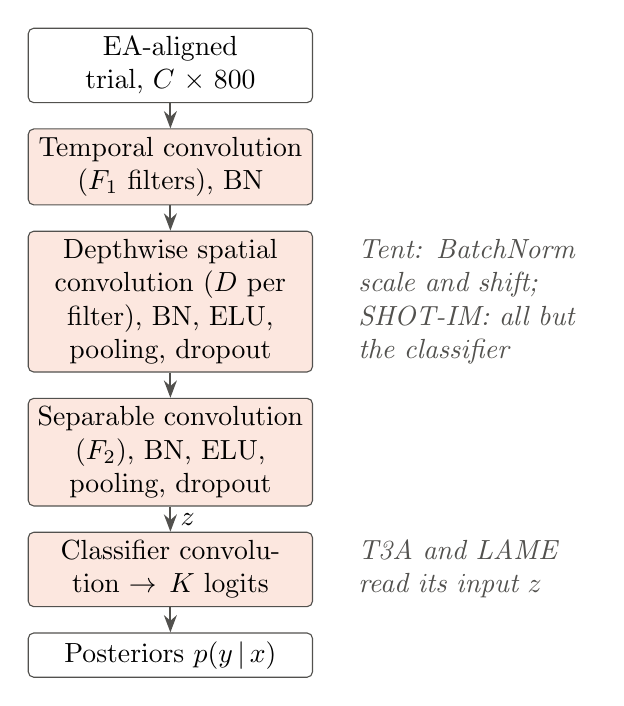
\begin{tikzpicture}[node distance=0.32cm]
\node[blk, text width=3.4cm] (x) {EA-aligned trial, $C\times800$};
\node[trn2, text width=3.4cm, below=of x] (t1) {Temporal convolution ($F_1$ filters), BN};
\node[trn2, text width=3.4cm, below=of t1] (t2) {Depthwise spatial convolution ($D$ per filter), BN, ELU, pooling, dropout};
\node[trn2, text width=3.4cm, below=of t2] (t3) {Separable convolution ($F_2$), BN, ELU, pooling, dropout};
\node[trn2, text width=3.4cm, below=of t3] (c2) {Classifier convolution $\to K$ logits};
\node[blk, text width=3.4cm, below=of c2] (p) {Posteriors $p(y\,|\,x)$};
\draw[arr] (x)--(t1); \draw[arr] (t1)--(t2); \draw[arr] (t2)--(t3);
\draw[arr] (t3)--node[right, font=\fontsize{10}{12}\selectfont]{$z$}(c2); \draw[arr] (c2)--(p);
\node[note, text width=2.9cm, right=0.45cm of t2] {Tent: BatchNorm scale and shift; SHOT-IM: all but the classifier};
\node[note, text width=2.9cm, right=0.45cm of c2] {T3A and LAME read its input $z$};
\end{tikzpicture}
\end{document}
